\tikzset{
	wordnode/.style = {circle,fill=black,inner sep=0,minimum size=4pt},
	arc/.style = {draw,  -latex'},
	decision/.style = {diamond, draw, fill=blue!20,
		text width=4.5em, text badly centered, node distance=3cm, inner sep=0pt},
	block/.style = {rectangle, draw, fill=blue!20,
		text width=3em, text centered, rounded corners, minimum height=4em},
	textdata/.style = {rectangle,
		text width=3em, text centered, minimum height=4em},
	procedure/.style = {rectangle, draw, fill=blue!20,
		text width=3.5em, text centered,  minimum height=3em,  minimum width=3em},
	line/.style = {draw,very thick,  -latex'},
	line1/.style = {draw, thick, dashed},
	compose/.style = {rectangle, draw, fill=none, rounded corners, blue, thick},
	cloud/.style = {draw, ellipse,fill=red!20, node distance=3cm,
		minimum height=2em},
	subroutine/.style = {draw,rectangle split,
		rectangle split parts=3,minimum height=1cm,
		rectangle split part fill={red!50, green!50, blue!20, yellow!50}},
	connector/.style = {draw,circle,node distance=3cm,fill=yellow!20},
	data/.style = {draw, trapezium, text width=3em, align=center, fill=olive!20, trapezium left angle=75pt, trapezium right angle=105, trapezium stretches = true, minimum height=3em, minimum width = 3em},
	mytrap/.style={trapezium, trapezium angle=67.5, draw, inner ysep=5pt, outer sep=0pt,  minimum height=1.81mm, minimum width=0pt}
}

\definecolor{a1c}{rgb}{0.00,0.00,1}
\definecolor{a2c}{rgb}{0.30,0.00,0.70}
\definecolor{a3c}{rgb}{0.00,0.50,0.50}
\definecolor{a4c}{rgb}{0.70,0.00,0.70}
\definecolor{a5c}{rgb}{1.00,0.00,0.00}
\definecolor{a6c}{rgb}{0.00,1.00,0.00}
\definecolor{a7c}{rgb}{0.20,0.60,0.20}
\definecolor{a2czy}{rgb}{1,0.9,0.6}
\definecolor{a10c}{rgb}{1, 0.75,0.4}
%\iffalse
%\begin{figure}[tb]
%\small
%%\begin{center}
%\begin{tikzpicture}[node distance = 0.35cm]
%
%\node [inner sep=0pt, left of = a1, node distance = 2.0em] (a0) {\$};
%
%\node [inner sep=0pt, right of = a1, node distance = 2.5em] (a2) {and};
%\node [inner sep=0pt, right of = a2, node distance = 2.5em] (a3) {UK};
%\node [inner sep=0pt, right of = a3, node distance = 3.5em] (a4) {Criticise};
%\node [inner sep=0pt, right of = a4, node distance = 4.5em] (a5) {Mugabe};
%\node [inner sep=0pt, right of = a5, node distance = 3em] (a6) {'s};
%\node [inner sep=0pt, right of = a6, node distance = 3em] (a7) {Victory};
%
%%gold ref
%\node [right of = a1, node distance = 2.5em] (a1-a3-m) {};
%\node [compose, black, fill = a2czy, opacity=.8, below of = a1-a3-m, minimum height = 1.5em,  minimum width = 6.8em, inner sep=0pt,  node distance = 1.5em]   (span-a1a3){Holder};
%\node [compose, black, fill = pink!80, opacity=.8, below of = a4, minimum height = 1.5em,  minimum width = 4.4em, inner sep=1pt,  node distance = 1.5em]   (span-a4){Expression};
%\node [compose, black, fill = green!50, opacity=.8, below of = a6, minimum height = 1.5em,  minimum width = 10.0em, inner sep=0pt,  node distance = 1.5em]   (){Target};
%
%\node [inner sep=0pt, above of = a0, node distance = 0.5em] (ba0) {};
%\node [inner sep=0pt, above of = a1, node distance = 0.5em] (ba1) {};
%\node [inner sep=0pt, right of = ba1, node distance = 0.5em] (rba1) {};
%
%\node [inner sep=0pt, above of = a2, node distance = 0.5em] (ba2) {};
%\node [inner sep=0pt, above of = a3, node distance = 0.5em] (ba3) {};
%
%\node [inner sep=0pt, above of = a4, node distance = 0.5em] (ba4) {};
%\node [inner sep=0pt, left of = ba4, node distance = 0.5em] (lba4) {};
%\node [inner sep=0pt, right of = ba4, node distance = 0.5em] (rba4) {};
%
%\node [inner sep=0pt, above of = a5, node distance = 0.5em] (ba5) {};
%\node [inner sep=0pt, right of = ba5, node distance = 0.5em] (rba5) {};
%\node [inner sep=0pt, above of = a6, node distance = 0.5em] (ba6) {};
%\node [inner sep=0pt, above of = a7, node distance = 0.5em] (ba7) {};
%\node [inner sep=0pt, left of = ba7, node distance = 0.5em] (lba7) {};
%
%
%
%\path [draw, thick, ->] (rba1) to [out=80, in=100] (ba2.north) {};
%\path [draw, thick,->] (rba1) to [out=80, in=95] (ba3.north) {};
%\path [draw, thick,->] (lba4) to [out=100, in=80] (ba1.north) {};
%
%
%\path [draw, thick, ->] (ba0) to [out=80, in=95] (ba4.north) {};
%\path [draw, thick, ->] (lba7) to [out=100, in=80] (ba5.north) {};
%\path [draw, thick, ->] (rba5) to [out=80, in=100] (ba6.north) {};
%
%\path [draw, thick, ->] (rba4) to [out=80, in=100] (ba7.north) {};
%
%\end{tikzpicture}
%%\end{center}
%\caption{Example of  ORL and dependency structures.
%}
%\label{graph:example}
%\end{figure}
%\fi

\begin{figure}[tb]
	\small
	
	%\begin{center}
	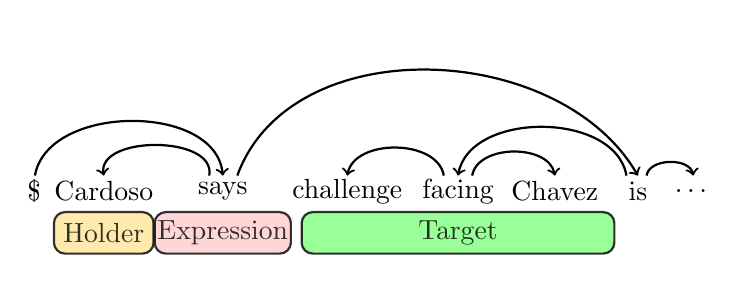
\begin{tikzpicture}
		\centering
		
		\node [inner sep=0pt] (a1) {Cardoso};
		\node [inner sep=0pt, left of = a1, node distance = 2.5em] (a0) {\$};
		\node [inner sep=2pt, right of = a1, node distance = 4.3em] (a2) {says};
		\node [inner sep=0pt, right of = a2, node distance = 4.5em] (a3) {challenge};
		\node [inner sep=0pt, right of = a3, node distance = 4em] (a4) {facing};
		\node [inner sep=0pt, right of = a4, node distance = 3.5em] (a5) {Chavez};
		\node [inner sep=0pt, right of = a5, node distance = 3.0em] (a6) {is};
		\node [inner sep=0pt, right of = a6, node distance = 2.0em] (a7) {…};
		
		
		%gold ref
		\node [compose, black, fill = a2czy, opacity=.8, below of = a1, minimum height = 1.5em,  minimum width = 3.6em, inner sep=0pt,  node distance = 1.5em]   (span-a1a3){Holder};
		\node [compose, black, fill = pink!80, opacity=.8, below of = a2, minimum height = 1.5em,  minimum width = 4.4em, inner sep=1pt,  node distance = 1.5em]   (span-a4){Expression};
		\node [compose, black, fill = green!50, opacity=.8, below of = a4, minimum height = 1.5em,  minimum width = 11.3em, inner sep=0pt,  node distance = 1.5em]   (){Target};
		
		\node [inner sep=0pt, above of = a0, node distance = 0.5em] (ba0) {};
		\node [inner sep=0pt, above of = a1, node distance = 0.5em] (ba1) {};
		
		\node [inner sep=0pt, above of = a2, node distance = 0.5em] (ba2) {};
		\node [inner sep=0pt, right of = ba2, node distance = 0.5em] (rba2) {};
		\node [inner sep=0pt, left of = ba2, node distance = 0.5em] (lba2) {};
		\node [inner sep=0pt, above of = a3, node distance = 0.5em] (ba3) {};
		
		\node [inner sep=0pt, above of = a4, node distance = 0.5em] (ba4) {};
		\node [inner sep=0pt, left of = ba4, node distance = 0.5em] (lba4) {};
		\node [inner sep=0pt, right of = ba4, node distance = 0.5em] (rba4) {};
		
		\node [inner sep=0pt, above of = a5, node distance = 0.5em] (ba5) {};
		\node [inner sep=0pt, right of = ba5, node distance = 0.5em] (rba5) {};
		\node [inner sep=0pt, above of = a6, node distance = 0.5em] (ba6) {};
		\node [inner sep=0pt, right of = ba6, node distance = 0.3em] (rba6) {};
		\node [inner sep=0pt, left of = ba6, node distance = 0.4em] (lba6) {};
		\node [inner sep=0pt, above of = a7, node distance = 0.5em] (ba7) {};
		\node [inner sep=0pt, left of = ba7, node distance = 0.5em] (lba7) {};
		
		
		
		\path [draw, thick, ->] (lba2) to [out=80, in=100] (ba1.north) {};
		\path [draw, thick,->] (ba0) to [out=80, in=95] (ba2.north) {};
		\path [draw, thick,->] (lba4) to [out=100, in=80] (ba3.north) {};
		
		\path [draw, thick, ->] (lba6) to [out=100, in=80] (ba4.north) {};
		\path [draw, thick, ->] (rba2) to [out=70, in=120] (ba6.north) {};
		
		\path [draw, thick, ->] (rba4) to [out=80, in=100] (ba5.north) {};
		\path [draw, thick, ->] (rba6) to [out=80, in=100] (ba7.north) {};
		
		
	\end{tikzpicture}
	%\end{center}
	\caption{An Example of ORL (bottom) and syntactic dependency tree (top) for ``Cardoso says challenge facing Chavezis is reestablishing normalcy.''
	}
	\label{graph:example}
\end{figure}
